\section{Research Approach}
This section presents the research methodology used in this thesis. First, the main purpose of the research and the research questions are presented. Furthermore, design research process including awareness of problem, suggestions and solutions, implementation, evaluation and conclusion is described. The section ends with list of validity threats that should be considered.  

\subsection{Research Purpose}
The purpose of this thesis is to investigate how a fault injection approach can help development teams at Ericsson to verify and test the fault tolerance abilities of the distributed systems (the Radio Base Station). The main characteristic of such systems is that they consist of small embedded components, whose computation power is very limited. Based on the experiences of such a fault injection approach, another research purpose of this thesis is how this approach can be generalized so that it can be adapted by companies who have the need to test embedded distributed systems, like the systems on the vehicles or airplanes.

\subsection{Research Question}
This section presents the questions that this thesis aims to answer.

\begin{description}
\item {\textbf{Main Question:}} 
\begin{itemize}
  
  \item Due to the limitations of traditional methods used by Ericsson for testing distributed systems, the high availability requirements of the products delivered by Ericsson, and the complexity of testing embedded distributed systems. The first research question is how to develop a fault injection approach for testing the robustness of the embedded distributed systems at Ericsson?
  
  \item As distributed systems is becoming more complex and the difficulty of testing the services that are running on large scale distributed systems, as well as the fault injection technique has been proposed as a possible way to address the fault tolerance challenges of distributed systems. The second research question is how the above approach can be utilized in other companies that have similar and common context? 
  
  \end{itemize}
  

\end{description}

\subsection{Research Methodology}
After a deep studying of different research methodologies together with our thesis context, the design and creation methodology was selected. Design and creation research was developed to address theoretical questions about the nature of learning in context. It is mainly used when a creation of new knowledge is seeking in order to solve a particular phenomenon through designing innovative artifact \cite{designresearch}. The phenomenon being investigated is mainly to verify the robustness of the RBS components at Ericsson as well as investigate the bottleneck of their distributed system. In order to address the problem that Ericsson has, a new artifact has been introduced and implemented using design and creation research methodology. After that, the new design was evaluated. Finally, a conclusion was carried out on how well the new model works and final results were presented. Rules and constraints were well identified for further use in studies with similar context. 
%\newline

The development process of this thesis was done in agile way. List of well specified requirements were identified with priorities. Work delivery was done in iterations. Considering that each iteration is three weeks. We started this thesis on the 19th of February, we used the first two weeks to get familiar with the PM framework. Each iteration took three working weeks, the first iteration was started on the 1st of March and ended on the 21th of March, the implementation was finished at the beginning of June. The work was done in four iterations. During the first iteration, we implemented the random messages sending, then we integrated the random messages sending into the automatic testing environment in the second iteration. Messages delaying was implemented during the third iteration and was integrated into the automatic testing environment in the last iteration.
%\newline

Weekly meeting with the supervisor from Ericsson for delivering what has done, getting feedback as well as planning for next iteration. Getting continuous feedback from the supervisors helped us in gaining more information about the system, discussing the obstacles, getting some suggestion and solutions, at the same time validating the work continuously. The following sections present the stages of the design and research process including awareness of the problem, suggestion and solution, implementation, evacuation and lastly the final conclusion as shown in Figure \ref{Design_Research_Process}. 

\begin{figure}
\centering
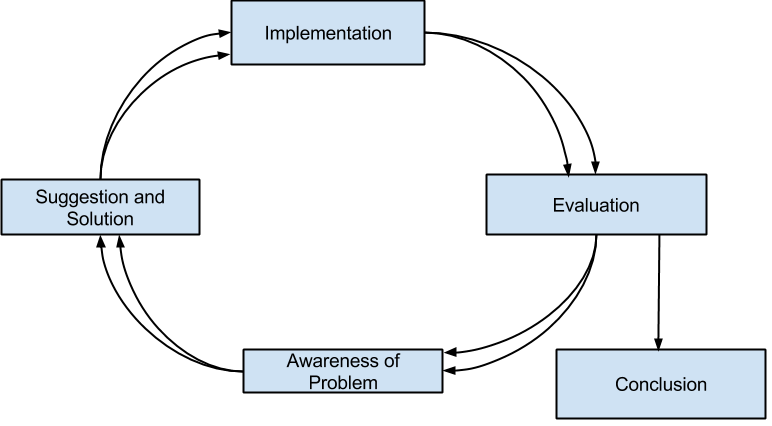
\includegraphics[width=150mm]{figure/Design_Research_Process.png}
\caption{Design Research Process \label{Design_Research_Process}}
\end{figure}
%\newpage

\subsubsection{Awareness of Problem}

The first strategy used in this phase was collecting information about different fault types through deep literature studying. By studying the previous related work, we took an inspiration for developing the new approach. Furthermore, we had meetings with the supervisors at Ericsson in order to gather more information on how the system works as well as some suggestions about the injection. We also analyzed Ericsson PM framework documents for identifying the bottleneck of the system and determining the injections.
%\newline

Additionally, Ericsson’s internal fault reports and other available documents helped in gathering more information about the weakness of the system and identifying where problems can occur. After deep studying of system weakness together with possible faults which might happen in reality, random faults were designed. At the same time the system was experimented by running with different scenarios and inspecting the log files.  
%\newline
 

\subsubsection{Suggestion and Solution}

The main strategies that we used in this phase were weekly meeting with the supervisor and observation. During the weekly meeting, the supervisor presented the PM framework and some libraries it uses. At the same time we consulted the supervisor regarding our doubts. Some suggestions were also proposed though our meetings with the supervisor. Observation includes reading the documents, the source code and log files of the PM framework. Getting feedback from the supervisor helped us on finding reasonable solutions on the obstacles that we met. Tracking the behaviour of the system through the log files also helped us on finding the reason behind undesirable system behaviours. 
%\newline

Based on Ericsson fault report and designed fault tolerant ability of the PM framework, potential fault types were discussed with the supervisor. We decided to have two fault types, the first one was sending random messages and the second one was delaying messages. In sending random messages, we got the idea from the supervisor in order to test the filter ability of the PM framework against random invalid messages. Delaying the messages were performed between the critical components of the PM framework where faults can occur.         


\subsubsection{Implementation}
This section describes the implementation of the fault injection tool. The implementation contains two steps: tool development and tool integration. The first step mainly concerns the work of development the fault injection tool using an Ericsson internal shared library called Inter Process Communication. The second step mainly concerns the work of integrating the developed tool into the automatic testing environment of the PM framework. Both fault development and fault integration are described in details in the implementation chapter. 
  
\subsubsection{Evaluation}
Evaluation is a very important phase in the development process. As a matter of fact, evaluation gives an indication of the conformance level of how the tool works. In this study tool evaluation included the following:   

\begin{itemize}
    \item Weekly meeting with the supervisor for getting feedback.
    \item Well identified requirements for the expected conformance level on how the tool should work.
    \item Continuous validation of the requirements.
    \item Observing the results of running the fault injection tool through the log files.
    \item Comparing the observed results with the expected (how the system should perform in its normal state). 
    \item If faults were detected, evaluating the faults by tracing back to the cause that made them.
\end{itemize}

The implementation of the fault injection tool was conducted in four iterations. During the first iteration, we implemented the random messages sending, then we integrated the random messages sending into the automatic testing environment in the second iteration. Messages delaying was implemented during the third iteration and was integrated into the automatic testing environment in the last iteration. Since we utilized agile development process, the fault injection approach was evaluated continually. Continuous evaluation of the approach helped us in developing the work as needed, decrease the uncertainty level, and increase the work quality. The source code of each iteration was pushed to the remote repository where the supervisor had access to it. During the weekly meeting, we got feedback from the supervisor of the fault injection tool. Furthermore, we presented the fault injection tool after the last iteration to the development team and got some feedback from them. 
%\newline

The faults caused by the new fault injection tool were monitored through log files, by analyzing the behaviors of the system through the log files, the new fault injection approach was evaluated continually. Everything appears in the log files introduced by the fault injection tool was analyzed in order to evaluate the tool. An example of unwanted system behavior can be like system interrupts, messaging delaying, timeout and so on.
%\newline

Model evaluation mainly depended on the results of running the fault injection tool. If the PM framework crashes after running the fault injection tool, the actual injection and the reason of the crashing will be evaluated first. If the random message sending triggers the PM framework crashing, the message types, contents, amounts and the frequency of the sending will be evaluated first. Based on the expected fault tolerant ability of the PM framework and the possible fault types which might exist in reality, some unnecessary provoking will be filtered out. For example, sending random message A with content B triggered the system crashing, but in reality, message A can never contain content B, then we just filter such a random message away. If sending message A with content C triggered some bugs in the PM framework, and in reality message A might contain content C, then we keep such a random message. 
%\newline

The fault injection approach works based on random manner, random selection can be both realistic and not in its nature. In order to get a reasonable indication of the approach evaluation, we made the input selection of the tool less randomized. By doing so, the approach is evaluated in a reasonable way and the results helped in discovering the unexpected faults. As a result, evaluating the detected faults helped us in evaluating the internal code as well as system architecture. After that, some suggestions were proposed on how internal code and architecture can be improved.     


\subsubsection{Conclusion}
This section describes the conclusion of system behavior after each fault injection scenario. Based on the running results of each iteration and continuous feedback from the supervisor as well as the development team, conclusion was constructed on how well the approach performed. Final evaluation of the approach mainly depended on final results of all iterations together.  
%\newline

After the final iteration, results were listed for the main research questions. Furthermore, the robustness and availability of the embedded distributed system were tested using the new fault injection approach. Conclusion was built on how well the approach worked, how did the system behave after fault injection and what are the keys of improvements for future work. As a conclusion of this study, we showed that fault injection technique can be applied to the embedded distributed system. Furthermore, unexpected faults were detected using this approach where non deterministic testing is applied. This approach also gave us well indication of the dependencies bottleneck where faults might occur, some keys of improvements were built from the observed results. Finally, this approach came as a complementary of the existing traditional testing approach.     
%\newline

\subsection{Validity Threats}
The validity of the study shows the trustworthiness of the final result and to which limit can the results be extended. Validity threats should not be biased by the researchers. Empirical research shows different thread to validity described in \cite{feldt2010validity}.This section shows the validity threats that were encountered during performing this study at the same time using different strategies in order to mitigate them. The threats were addressed not only at the final phase, but also during all the phases of the design research, in order to mitigate the risk of having unreliable results as much as possible \cite{guidelines}.
%\newline

\subsubsection{Internal validity}
Internal validity concerns about the causal relation between different factors when doing the testing. Factors can be the time that the faults were triggered, fault types, a combination of different fault types at different time, etc. Those factors have a causal relation in a way that they affect each others as well as the final result of testing \cite{experimentation}. %\newline

Internal validity can also be how well the factors were considered when doing the test. The following questions should be considered when doing internal validity. Were all the factors considered? Could some factors impact on the reliability of the result? Were there any factors that should be triggered in order to make other factors work? List of internal validity including history, maturation and ambiguity about direction of causal influence are described as the following: 
%\newline

\textbf{History:} Doing the same test at the same object but on different time when running the fault injection tool on the real environment can have different results. For instance, when the testing happened on a normal day or when it happened on a holiday considering the number of events that can happen are varies from day to another. This could be due to the fact that the circumstances were not the same on both occasions. To mitigate this threat, the test should be repeated at different time to assure the result reliability. All test cases on this study were done on the simulator and not on the real environment. For this reason, there will be a risk of not having the same result when doing it on the real environment.
%\newline

\textbf{Maturation:} This can be when the subject reacts differently over time. For instance, when the software scale over the time and the object relations become more complex, the behavior of the object could also change. When developing the fault injection tool, the XML messages name and message types were hard coded. Since part of the code were hard coded, does this have any effects when system scale. Ericsson distributed system can scale exponentially over time. Since we are doing the testing on small distributed system, being confident on that the testing technique will scale is very important. Having such scalable technique is a big challenge in software industry. Random testing can scale much better than other testing techniques on large systems and thus become more cost-effective on the long term \cite{random}. Utilizing random testing technique in this case will mitigate maturation threat.
%\newline

\textbf{Ambiguity about direction of causal influence:} 
Ambiguity about direction of causal influence is the difficulty to determine the causal relation between variables. In case of fault happened, it can be hard to verify the cause of it. When having a large and complex system identifying the causal relationship between the variable is not trivial task. For instance if A causes B or B causes A or even an external X causes A and B. When the fault injection implementation was integrated to the automatic testing environment, some of the injection which was ran manually triggered the crash of the automatic testing environment. This happened because of the strict dependencies in the automatic testing environment. The more complex the system is, the more ambiguous causal relation will be. Well understanding of the distributed system, the correlation between the components and dependencies will mitigate from this threat. 


\subsubsection{External Validity}
This section points out how much can the result be generalized. There are a lot of things should be considered when it comes to generalizing the model. The external validity cares about to which extend the result can be generalized. The main concerns is how to make the result general as much as possible so it can work on other similar environmental setting. \cite{experimentation}.
%\newline

\textbf{Interaction of selection and treatment:} 
This case can be when it comes to generalizing, having subjective populations that are not representative of the population, for instance when selecting just  programmers in an inspection experiments when programmers, testers, and system engineer should take part of the inspection. When doing the testing in this thesis different members were involved, including software developer, tester, software engineer, as well as supervisors from the academy in order to make the study objective as much as possible. However, when experimenting the test, the tester can insert some values into the variables on the configuration file such as number of messages, message types and time interval. By letting the user inserting those values, the result of the test can be biased. 
%\newline

\textbf{Interaction of setting and treatments:}
When doing the testing on toy environment not on a real environment. In our case doing the testing on the simulator instead of doing it on the real environments. Will the results be affected or changed?  
%\newline

\subsubsection{Conclusion validity}
This validity threat focus on the relationship between the treatment and the outcome. List of the conclusion validity is described in the following:
%\newline

\textbf{Fishing and the error rate:}
This study aims to detect at least single fault by fishing through random extermination. But on the other side this can not verify that fishing could generalize the reliability of the measurements.  
%\newline

\textbf{Reliability of measures:}
By experimenting the test more than once, we assured the reliability of the results. We got the same result at each time we repeat the experiment. 


\subsubsection{Construct validity}
Construct validity is focusing on how well the design constructed when doing the experiment (Testing). Moreover, this threat focuses more about does the result of the study covers the purpose as well as the research questions. In order to mitigate this threat the rules should be well identified at the same time the result should not be interpreted in a wrong way. 

\subsubsection{Reliability}
The main focus of this section is to identify how reliable is the final result. Will the results be effected if the experiments repeated again and again at different time or environments. Furthermore, in case of conducting the study by other researchers, will they come up with the same results \cite{guidelines}. In order to mitigate from this threat we have listed the rules needed to conduct the study at different companies with similar context. Moreover, as a non-expert of Ericsson embedded distributed system, gray box testing is performed by randomizing different test cases at different times. In this case, predicting unexpected faults will increase. Random testing seems to be more unbiased and has higher faults predictability than other testing techniques \cite{random}. Finally, by taking guidance and feedback from an external developers and researchers in both Ericsson and Chalmers, this will increase the unbiased judgment as well as the reliability of the results.

